\documentclass{standalone}
\usepackage{graphicx}	
\usepackage{amssymb, amsmath}
\usepackage{color}

\usepackage{tikz}
\usetikzlibrary{arrows.meta, backgrounds, math}
\usepackage{pgfmath}

\definecolor{light}{RGB}{220, 188, 188}
\definecolor{mid}{RGB}{185, 124, 124}
\definecolor{dark}{RGB}{143, 39, 39}
\definecolor{highlight}{RGB}{180, 31, 180}
\definecolor{light_teal}{RGB}{107, 142, 142}
\definecolor{mid_teal}{RGB}{72, 117, 117}
\definecolor{dark_teal}{RGB}{29, 79, 79}
\definecolor{gray10}{gray}{0.1}
\definecolor{gray20}{gray}{0.2}
\definecolor{gray30}{gray}{0.3}
\definecolor{gray40}{gray}{0.4}
\definecolor{gray60}{gray}{0.6}
\definecolor{gray70}{gray}{0.7}
\definecolor{gray80}{gray}{0.8}
\definecolor{gray90}{gray}{0.9}
\definecolor{gray95}{gray}{0.95}

\begin{document}

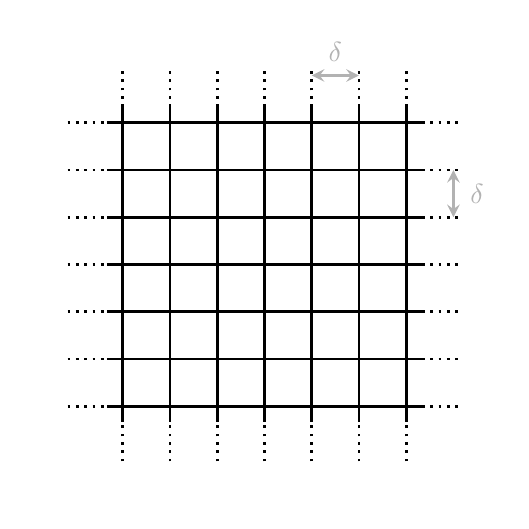
\begin{tikzpicture}[scale=1.0]

  \draw[white] (-3, -3) rectangle (3, 3);
  
  \foreach \y in { -1.8, -1.2, ..., 1.81 } {
    \draw[black, line width=1] (-2, \y) -- (2, \y);
    \draw[black, dotted, line width=1] (-2.5, \y) -- (-2, \y);
    \draw[black, dotted, line width=1] (2, \y) -- (2.5, \y);
  }
    
  \foreach \x in { -1.8, -1.2, ..., 1.81 } {
    \draw[black, line width=1] (\x, -2) -- (\x, 2);
    \draw[black, dotted, line width=1] (\x, -2.5) -- (\x, -2);
    \draw[black, dotted, line width=1] (\x, 2) -- (\x, 2.5);
  }
  
  \draw[gray70, <->, >=stealth, line width=1] (0.6, 2.4) -- (1.2, 2.4);
  \node[gray70] at (0.9, 2.7) { $\delta$ };

  \draw[gray70, <->, >=stealth, line width=1] (2.4, 0.6) -- (2.4, 1.2);
  \node[gray70] at (2.7, 0.9) { $\delta$ };
    
\end{tikzpicture}

\end{document}  